\documentclass{article}
\usepackage[polish]{babel}
\usepackage[utf8]{inputenc}
\usepackage[T1]{fontenc}
\usepackage{graphicx}
\usepackage{anysize}
\usepackage{enumerate}
\usepackage{times}
\usepackage{amsmath}

\usepackage{natbib}
\usepackage{graphicx}
\setcounter{section}{3}
\begin{document}

\section{Opracowanie wyników pomiaru}
    \subsection{}
    
         Obliczenie odchylenia standardowego $\sigma$ i sprawdzenie czy któryś z wyników jest odległy o więcej niż 3 $\sigma$:
        \[
        \sigma= \sqrt{\frac{(x_{1}-\bar{x})^{2}+(x_{2}-\bar{x})^{2}+...+(x_{n}-\bar{x})^{2}}{n-1}}
        \]
        Po podstawieniu wyznaczonych okresów, $3\sigma$ = 0.12 wynika z tego, że błędy grube nie wystąpiły.
    \subsection{}
        Obliczenie niepewności pomiaru okresu (typu A):
        \[
        u(x) = \sqrt{\frac{\sum(x-\bar{x})^{2}} {n(n-1)}}
        \]
        Po przeliczeniu:
        \[
        u(T) = 0.01227
        \]
    \subsection{}
        Ocenienie niepewności pomiaru okresu wachadła (typu B):
        \[
        u(l) = 1mm = 0.001m 
        \]
    \subsection{}
        Obliczenie przyspieszenia ziemskiego na podstawie $l$ i $T$:
        \[
        T=2\pi\sqrt{\frac{l}{g}} \Rightarrow g_p=4\pi^{2}\frac{l}{T^{2}} = 9.76\frac{m}{s^2}
        \]
    \subsection{}
        Obliczenie niepewności złożonej:
        \[
        u_{c}(y)= \sqrt{\sum_k\left[\frac{\partial{}y}{\partial{}x_{k}}u(x_{k})\right]^2}
        \]
        Więc dla wzoru na przyspieszenie ziemskie otrzymam:
        \begin{equation}
        \begin{split}
        u_{c}(g) &= \sqrt{\left(\frac{\partial{}g}{\partial{}T}u(T)\right)^2 + \left(\frac{\partial{}g}{\partial{}l}u(l)\right)^2} = \sqrt{\left(-8\pi^{2}\frac{l}{T^{3}}\cdot{}0.01227\right)^2 + \left(\frac{4\pi^{2}}{T^{2}}\cdot{}0.001\right)^2} = \\ &=\sqrt{\left(-8\pi^{2}\frac{1.1}{2.10^{3}}\cdot{}0.01227\right)^2 + \left(\frac{4\pi^{2}}{2.10^{2}}\cdot{}0.001\right)^2} = 0.1152
        \end{split}
        \end{equation}
    \subsection{}
        Obliczenie niepewności rozszerzonej (dla k=2):
        \[
        U(g)= k\cdot{}u_{c}(g) = 2\cdot{}0.1152 = 0.2304
        \]
    \subsection{}
        Obliczone wcześniej przyspieszenie ziemskie $g_p = 9.76\frac{m}{s^2}$ znajduje się w przedziale $(9.811\frac{m}{s^2} \pm 0.2304\frac{m}{s^2})$:
    \subsection{}
        Wykres zależności okresu od długości wachadła:
        \begin{figure}[h]
        \centering
        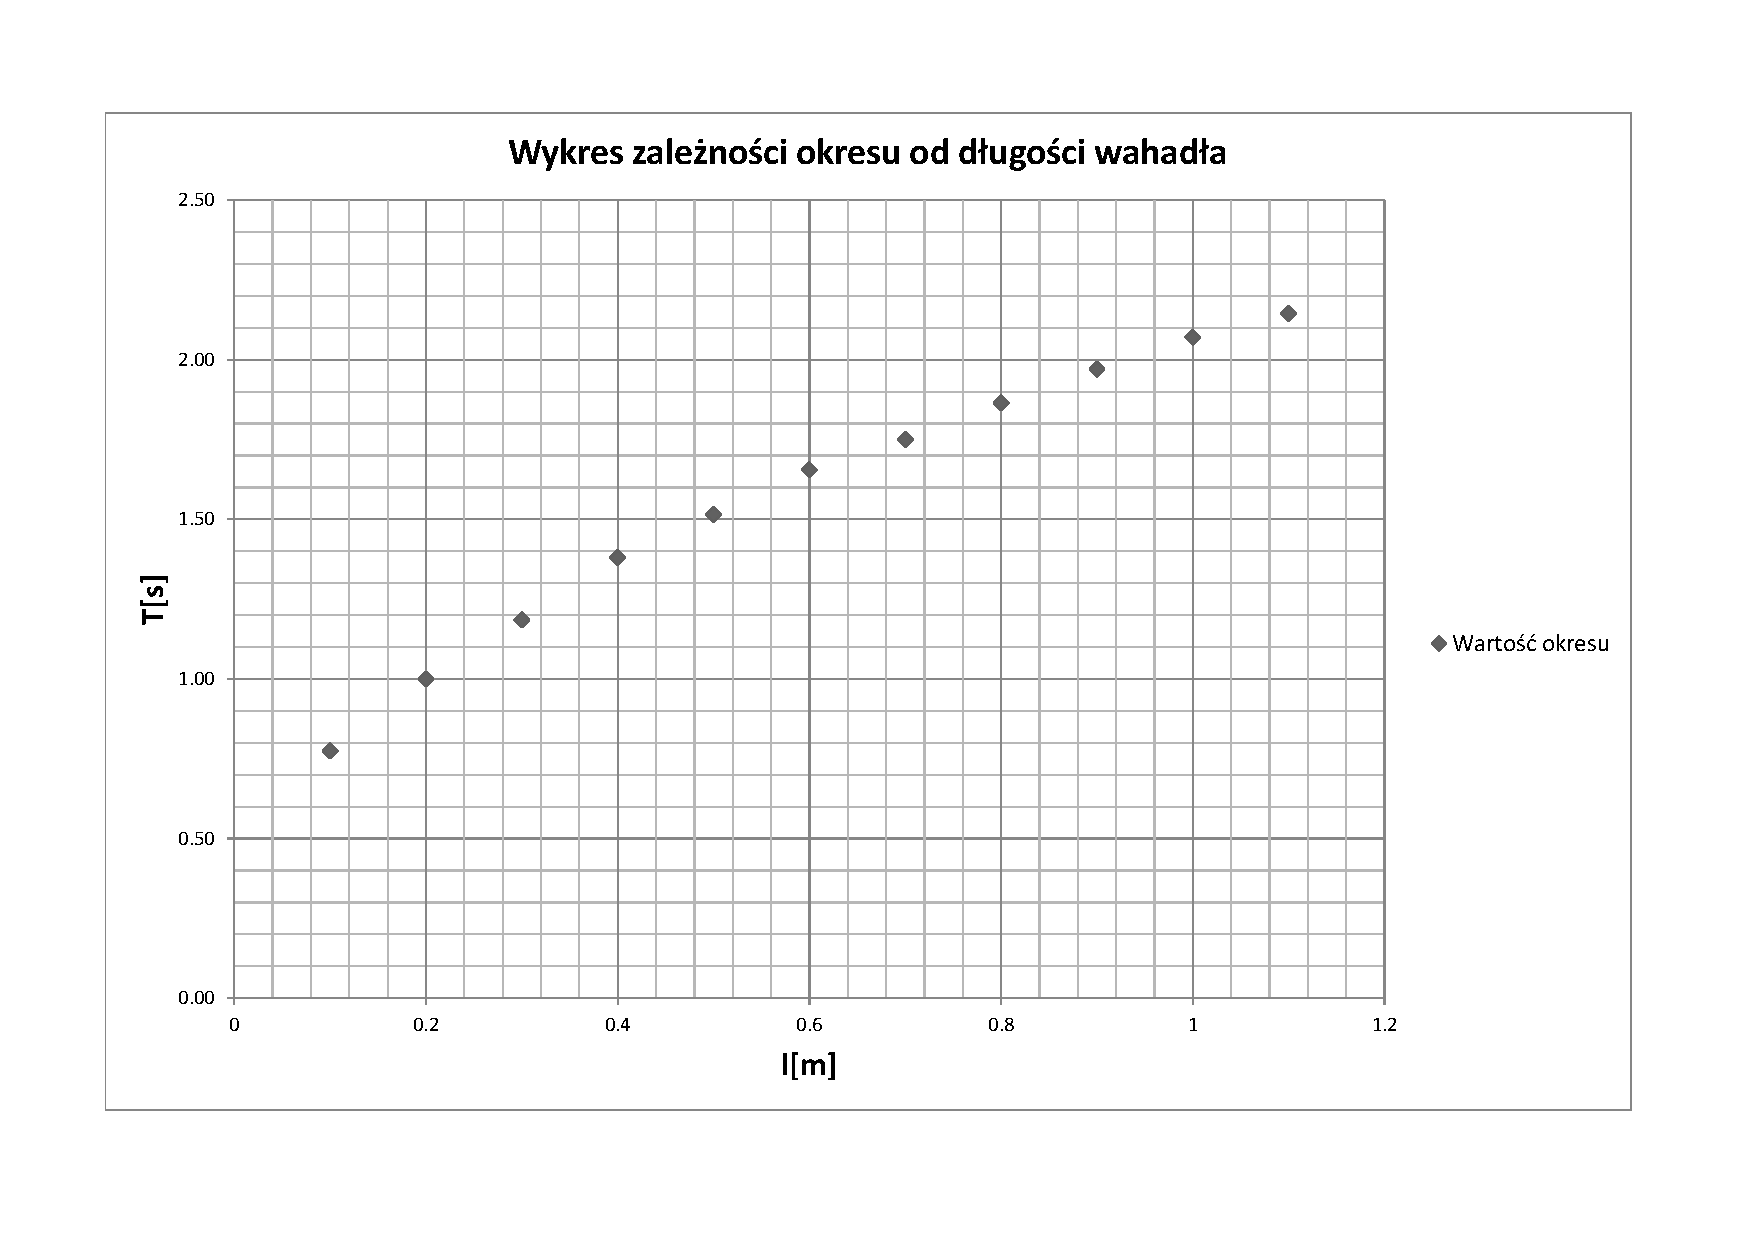
\includegraphics[width=0.9 \textwidth]{wykres3.pdf}
        \label{fig:wyk1}
        \end{figure}\newpage
    \subsection{}
        Zlinearyzowany wykres dla kwadratu okresu:
        \[
            T^{2}=4\pi{}^{2}\frac{l}{g} \Rightarrow T^{2}(l)=\frac{4\pi{}^{2}}{g}l
        \]
        \begin{figure}[h]
        \centering
        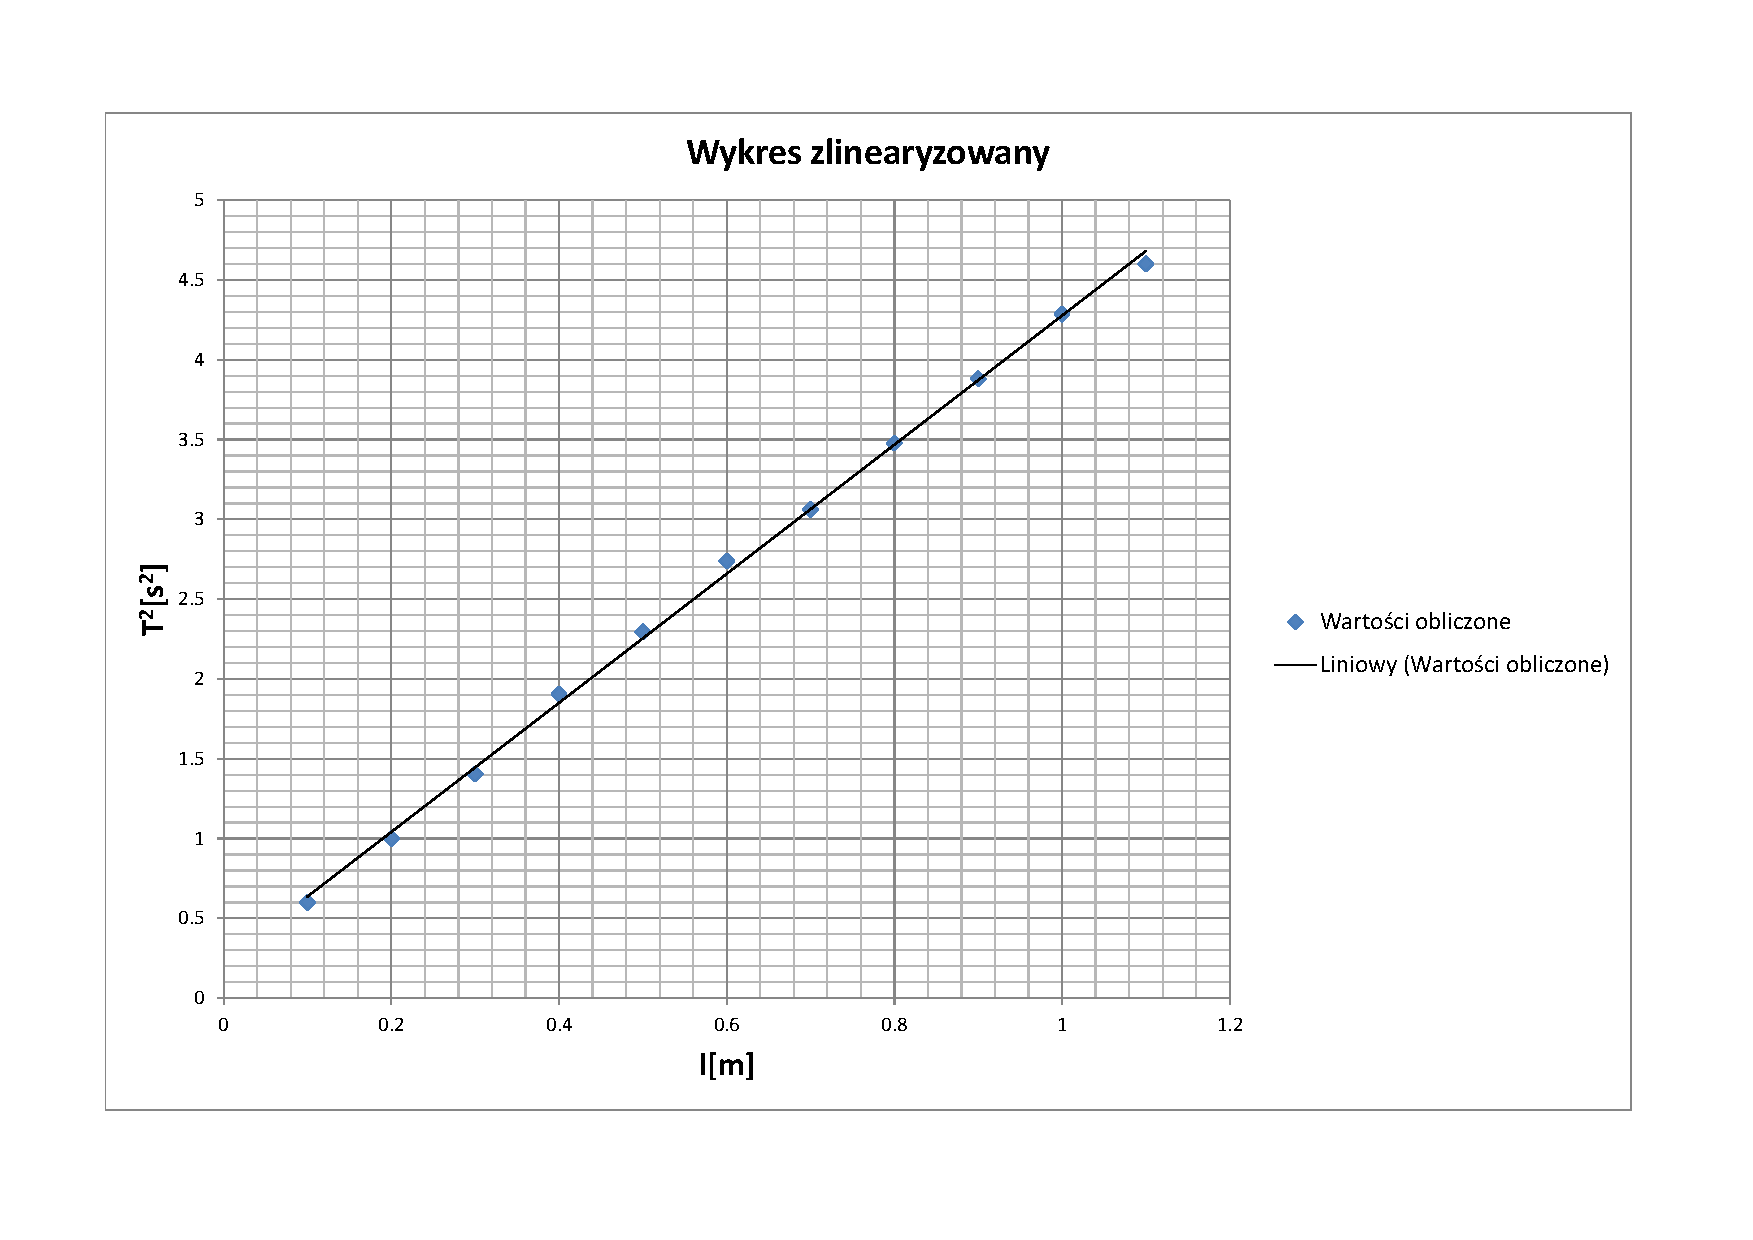
\includegraphics[width=1 \textwidth]{wykres4.pdf}
        \label{fig:wyk2}
        \end{figure}
    \subsection{}
        Korzystając z funkcji programu Microsoft Excel obliczam $a=4.04$ otrzymuję więc równanie prostej 
        \[
            y(x)=4.04x
        \]
    \subsection{}
        Korzystając z wzoru: 
        \[
            a=4\pi{}^{2}/g
        \]
        wyznaczam g:
        \[
            g=4\pi{}^{2}/a
        \]
        i po podstawieniu otrzymuję:
        \[
            g=4\pi{}^{2}/4.04 = 9.75\frac{m}{s^2}
        \]\newpage
    \section{Wnioski}
    Wartość przyspieszenia ziemskiego otrzymana za pomocą pomiarów okresów drgań wahadła dla jego stałej długości jest zgodna z wartością uzyskaną z pomiarów okresów drgania dla różnych długości wahadła, dla obliczonej niepewności rozszerzonej. Świadczy to o prawidłowym przeprowadzeniu pomiarów.
Oba wyniki są zaniżone, może to być spowodowane czynnikami zewnętrznymi takimi jak tarcie nitki oraz opory powietrza. Niedoskonały wynik jest również spowodowany faktem uproszczenia jakim jest założenie, że wahadło jest matematyczne, a takiego wahadła nie da się skonstruować w świecie rzeczywistym.

        
        

\end{document}
